\bibliographystyle{plain}
\section{Parametrization of the functions}

As we said above, the functions $f$ and $g$ must be parametrized.
The authors propose the following parametrizations for $f$ and $g$ :

\begin{align*}
  f(x,u) &= \sum_{i=1}^I \rho_i(x) h_i + Ax + Bu + b\\
  g(x,u) &= \sum_{j=1}^J \rho'_j(x) k_j + Cx + Du + d\\
  \rho_i(x) \colon \mathbb{R}^p &\to \mathbb{R}\\
  x &\mapsto \frac{1}{(2\pi)^{d/2}|S_i|^{1/2}} \exp \left(-\frac{1}{2}(x-c_i)^T S_{i}^{-1}(x-c_i)\right)\\
  \rho'_j(x) \colon \mathbb{R}^p &\to \mathbb{R}\\
  x &\mapsto \frac{1}{(2\pi)^{d/2}|S'_j|^{1/2}} \exp \left(-\frac{1}{2}(x-c'_j)^T {S'_{j}}^{-1}(x-c'_j)\right)\\
  A \in \mathbb{R}^{p \times p}, & \  B \in \mathbb{R}^{p \times q}, \  C \in \mathbb{R}^{n \times p}, \  D \in \mathbb{R}^{n \times q}\\
  h_i \in \mathbb{R}^{p},& \  b \in \mathbb{R}^p, \  k_j \in \mathbb{R}^{n},\   d \in \mathbb{R}^n\\
\end{align*}

The real valued functions $\rho_i$ and $\rho'_j$ are called radial basis functions (RBF).
The centers $c_i$ and $c'_j$ of the RBF are supposed to be known, as well as the width $S_i$ and $S'_j$.
We will see further that they can be learnt but, for the moment, we suppose that they are known.


So $f$ is the sum of an affine function ($x \rightarrow Ax + b$) and $I$ radial basis functions ($x \mapsto \rho_i(x) h_i$, $i=1 \cdots I$).
The parameters $\theta_f$ and $\theta_g$ of our functions are :

\begin{align*}
  \theta_f &= \left( h_1, \ldots , h_I, A, B, b\right) \\
  \theta_g &= \left( k_1, \ldots , k_J, C, D, d\right) \\
\end{align*}

If use no inputs and set the state dimension to 1 ($n = 1$), $f : \mathbb{R} \to \mathbb{R}$ can have the following form on the segment $\left [ 0 , 1 \right ]$:

\begin{figure}[H]
\captionsetup{labelformat=empty}
\minipage{0.32\textwidth}
  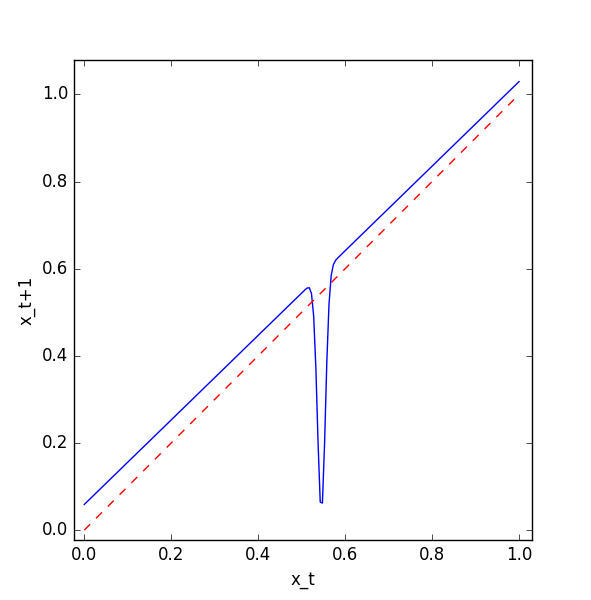
\includegraphics[width=\linewidth]{function_RBF_3.png}
  \caption{I = 1}
\endminipage\hfill
\minipage{0.32\textwidth}
  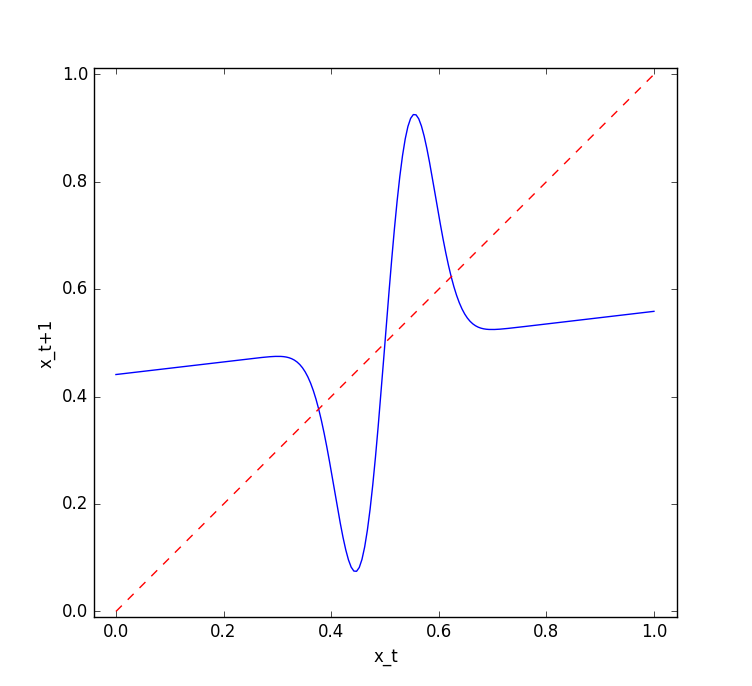
\includegraphics[width=\linewidth]{function_RBF_1.png}
  \caption{I = 2}
\endminipage\hfill
\minipage{0.32\textwidth}
  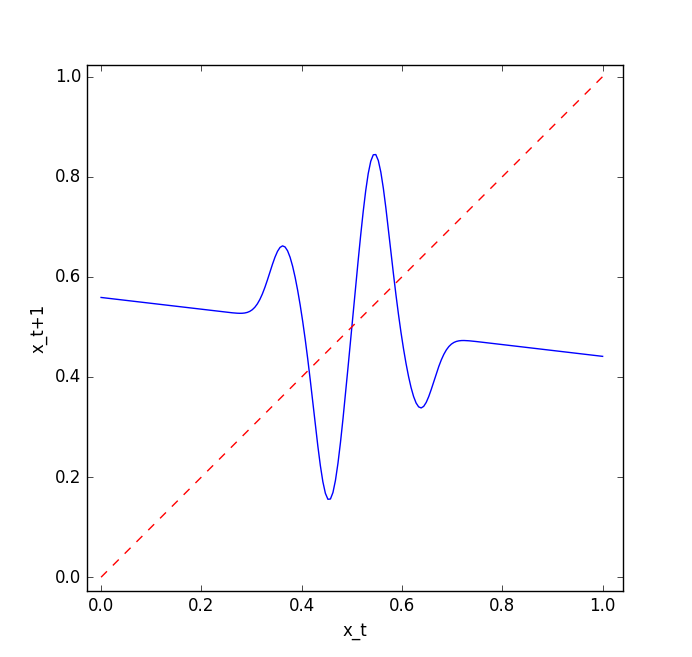
\includegraphics[width=\linewidth]{function_RBF_2.png}
  \caption{I = 4}
\endminipage\hfill
\end{figure}

Now that the functions $f$ and $g$ are parametrized, we can begin with the study of the proposed EM algorithm.
